\documentclass{standalone}
\usepackage{tikz}
\usepackage{ctex,siunitx}
\usepackage{tkz-euclide}
\usepackage{amsmath}
\usetikzlibrary{patterns, calc}
\usetikzlibrary {decorations.pathmorphing, decorations.pathreplacing, decorations.shapes,}
\begin{document}
\small
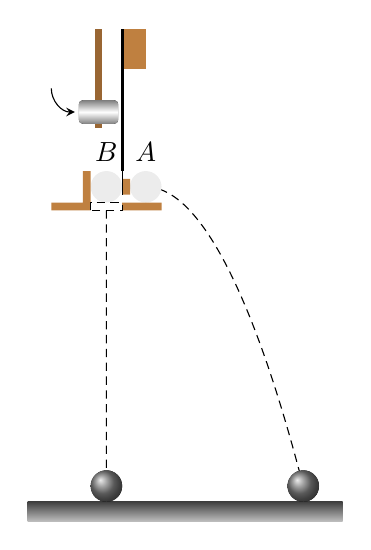
\begin{tikzpicture}[>=stealth,scale=1.0]
  \fill[top color=darkgray,bottom color=lightgray](-1,0)rectangle(3,-0.25);
  \draw[densely dashed](0.5,4)parabola(2.5,0.2)(0,3.7)--(0,0.2);
  \fill[ball color=gray] (0,0.2)circle(0.2);
  \fill[ball color=gray] (2.5,0.2)circle(0.2);
  \fill[fill=lightgray!30](0,4)circle(0.2)node[above=2mm]{$B$}(0.5,4)circle(0.2)node[above=2mm]{$A$};
  \fill[brown](0.2,3.7)rectangle++(0.5,0.1)(0.2,3.9)rectangle++(0.1,0.2)(-0.2,3.7)rectangle++(-0.5,0.1)(-0.2,3.7)rectangle++(-0.1,0.5);
  \draw[very thin,densely dashed](-0.2,3.7)rectangle++(0.4,0.1);
  \draw[ultra thin](0.2,3.9)--(0.2,4.2);
  \fill[brown](0.2,6)rectangle++(0.3,-0.5);
  \draw[very thick](0.2,6)--(0.2,4.2);
  \fill[brown!80!black](-0.05,4.75)rectangle(-0.15,6);
  \fill[rounded corners=0.5mm,top color=gray,bottom color=gray,middle color=white](-0.35,5.1)rectangle(0.15,4.8);
  \draw[<-,thin](-0.4,4.95)arc(270:180:0.3);
\end{tikzpicture}
\end{document}